\documentclass[]{article}
\usepackage{caption}
\usepackage{tocloft}
\usepackage{amssymb,amsmath}
\usepackage{ifxetex,ifluatex}
\usepackage{fixltx2e} % provides \textsubscript

\usepackage{longtable}
\usepackage{graphicx}
\usepackage{tikz}

\setlength{\parindent}{0pt}
\setlength{\parskip}{6pt plus 2pt minus 1pt}
\setlength{\emergencystretch}{3em}  % prevent overfull lines
\setcounter{secnumdepth}{0}

\usepackage[left=1.5in,right=1.5in]{geometry}
\usepackage{float}
\floatplacement{figure}{h}

\usepackage{sectsty}
\usepackage[normalem]{ulem}
\sectionfont{\rmfamily\bfseries\large}
\subsectionfont{\rmfamily\centering\upshape\normalsize}
\subsubsectionfont{\centering\normalsize}

\fontsize 12
\usepackage{hyperref}
\usepackage{lineno}
\linenumbers
\usepackage[font={footnotesize,sf}]{caption}
\usepackage{siunitx}

\usepackage{setspace}
\linespread{1.5}

\raggedbottom

\usepackage{titling}
\pretitle{\begin{flushleft}\Large\bfseries}
\posttitle{\end{flushleft}}
\preauthor{\begin{flushleft}\large}
\postauthor{\end{flushleft}}
\predate{\begin{flushleft}\large}
\postdate{\end{flushleft}}


\usepackage{fancyhdr}
\pagestyle{fancy}
\lhead{  \nouppercase  \leftmark}
\rhead{\thepage}
\cfoot{}

\hypersetup{breaklinks=true,
            bookmarks=true,
            colorlinks=true,
            citecolor=blue,
            urlcolor=blue,
            linkcolor=magenta,
            pdfborder={0 0 0}}
\urlstyle{same}  % don't use monospace font for urls

\usepackage{authblk}

\title{Phase Transitions in Landscape Connectivity}
\author[1,2]{M.D. Catchen}
\author[1]{S.M. Flaxman}
\affil[1]{\small{Department of Ecology and Evolutionary Biology, University of Colorado at Boulder}}
\affil[2]{\small{Department of Biology, McGill University}}
\date{\today}


\usepackage[square, numbers]{natbib}
\bibliographystyle{unsrtnat}
\begin{document}
\maketitle
\begin{abstract}

dang ol absrtact here

\end{abstract}
\clearpage

\section{Introduction}

Landscape connectivity intro

Ecological processes are inherently the product of interactions across all scales of biological organization \cite{levin_problem_1992}. This process of \textit{emergence}, by which parts come together to form a whole with properties that don't exist among the individual parts, has been studied across a wide variety of disciplines \cite{manrubia_emergence_2004} and is a ubiquitous phenomenon in complex systems. One potential cause of emergent behavior is \textit{synchrony} among the individual parts of a complex system. When many independent parts come together to act as a whole, their dynamics become synchronized.
This behavior is ubiquitous in biological systems across all scale of organization.
From collections of cells acting together: the heart beating in rhythm \cite{womelsdorf_modulation_2007}, neurons firing in unison \cite{strogatz_sync_2003}---to behavior among organisms: the flash of fireflies \cite{otte_theories_1980} or the migration of birds \cite{spottiswoode_extrapair_2004}---to interactions between organisms: synchrony between abundances of predators and prey \cite{lv}, and of phenology \cite{van_asch_phenology_2007,burkle_future_2011}.
Synchrony, by definition, involves different entities changing over time in the same way. Within ecology, there has long been a focus on spatial synchrony, that is—how does spatial distribution of ecological entities affect whether they change together or separately? \cite{jarillo_spatial_2020, kendall_dispersal_2000, hanski_spatial_1993}.
This is, in large part, due to the applied importance of understanding the effect of habitat loss on natural populations. Many theoretical studies have shown the two primary factors that develop spatial synchrony across space are dispersal and environmental covariance \cite{ripa_analysing_2000, abbott_does_2007}.
Within this theory, one maxim that has developed is \textit{Moran's rule}, which states that spatial synchrony is proportional to the covariance in the environmental conditions across space \cite{ranta_synchrony_1995, bjornstad_spatial_1999}.


A major goal of conservation is developing corridors to conserve
landscape connectivity. Most measures of landscape connectivity used in the literature represent \emph{structural} connectivity, meaning quantifying the
structure of the landscape \cite{}. Structural connectivity stands in constract with \emph{functional} connectivity, which measures the connectivity of a given process \cite{kool_population_2013, calabrese_comparison-shoppers_2004}. Here,
in order to better understand functional connectivity, we use a
simulation model to measure how synchrony across space changes as a
function of landscape structure. We do this by developing a model of
metapopulation dynamics on spatial graphs, which have long been used to
model landscape connectivity \cite{martensen_spatio-temporal_2017,
@albert_applying_2017, @urban_landscape_2001}, and analyze how
synchrony changes across space using the language of critical
transitions.

Further, we show that increasing population synchrony reduces the
variance in the generation-to-generation change in abundance, which is
central in reducing the probability of metapopulation extinction
(@lande\_risks\_1993, @lande\_extinction\_1998). This relationship
suggests that promoting functional landscape connectivity can help
mediate the probability of extinction for species facing significant
habitat loss. We suggest using simulation models, such as those
presented here, to aid in decision making regarding corridor placement.

\section{What are phase transitions?}


\hypertarget{what-are-phase-transitions}{%
\subsection{What are phase
transitions?}\label{what-are-phase-transitions}}

When does a system change from one state to a different state? Due to
the rapid changes induced on the planet by human activity, there has
been recent focus on answering this question in ecology, especially the
potential for changes in spatial structure to drive transitions between
alternative stable states. Much of this theory has been aimed at the
practical problem of being able to predicting the onset of transitions
from time-series data \cite{scheffer_anticipating_2012, scheffer_early-warning_2009}. The bulk of the quantitative theory
used to understand transitions between states is derived from
statistical mechanics, where it was originally used to study
phase-transitions in matter. In order to study phase transitions between
regimes, we must first be clear on what these regimes are. As this
theory was originally used to describe physical states of matter, the
original regimes were solid, liquid, gas. However, as our understanding
of condensed-matter has changed, so has the demarcation of what
constitutes different states. In reality, the way in which particles
come together to constitute matter is far more variable than these three
categories. In such cases the `state' of a collection of particles
cannot be represented by a single categorical label, and so the theory
of phase transitions as been adapted to model \emph{continuous} phase
transitions, where there is no clear demarcation point between different
states \cite{sethna_statistical_2006}. This is useful for us in ecology,
where the line between alternative ecosystem `states' is even fuzzier.

We can formalize our understanding of phase transitions using the
language of statistical mechanics. We call the \emph{order parameter}
some measure of the system's state in space and time. The \emph{control
parameter}, then, is what causes the change in order parameter. When
dealing with dynamics that are inherently stochastic, one tool often
used in statistical mechanics is correlation functions which measure how
well the order parameter is correlated in both space and time at a
particular value of the control parameter \cite{sethna_statistical_2006}.
For example, if we consider the population of a species inhabiting a
landscape, where along the gradient of landscape connectivity, our
control parameter, does that system go from consisting of one large,
single, population, to many small, independent populations? We measure
this qualitative shift from one system to many using \emph{synchrony},
the correlation in the dynamics of abundance across space.

\pagebreak

\hypertarget{the-model}{%
\section{The Model}\label{the-model}}

Here we present a spatial graph model of landscape connectivity based on
metapopulation theory \cite{hanski_practical_1994, grilli_metapopulation_2015} . We model connectivity as a function of
a few empirically estimable parameters, and then describe a stochastic
model of metapopulation dynamics on these spatial graphs. We then
simulate dynamics across a gradient of landscape
connectivity parameters to measure transitions in the synchrony of
population dynamics across space occur.

\hypertarget{modeling-landscape-connectivity-with-a-spatial-graph}{%
\subsection{Modeling Landscape Connectivity with a Spatial
Graph}\label{modeling-landscape-connectivity-with-a-spatial-graph}}

Spatial graphs have long been used to model a system of habitat patches
\cite{dale_graphs_2010, minor_graph-theory_2008,
urban_landscape_2001}. Here we model a system of populations, represented as a vector of
vertices, $\vec{L}$ in a spatial graph \(G=(L,E)\). Here the edges \(E\)  represent dispersal between populations. To define $E$,  we choose to model landscape connectivity with respect to the process of metapopulation dynamics as a combination of two different factors: the probability than any individual migrates during its lifetime, $m$, and the conditional distribution over spatial nodes of where an individual goes, given that
it migrates, \(P(L_j|L_i)\), which we call the dispersal potential, $\Phi_{ij}$. We can model the dispersal potential using a few methods. In empirical
systems, this can be estimated with resistance surfaces, which provide
relative weights of the difficulty of migration between points on a
raster of land-cover type \cite{spear_use_2010}. Theoretically, we model
the dispersal potential using isolation-by-distance (IBD). The relative
probability of dispersal between \(L_i\) to \(L_j\) is inversely
proportional to the distance between them, \(d_{ij}\), and the strength
of this isolation-by-distance relationship, \(\alpha\). The
functional form of this relationship, \(f(d_{ij}, \alpha)\), has long been called the dispersal kernel \cite{hanski_practical_1994}.
Here we consider two different types of dispersal kernels: the
exponential, \(f(d_{ij}, \alpha)=e^{-\alpha d_{ij}}\), and
Gaussian, \(f(d_{ij}, \alpha)=e^{-\alpha^2 d_{ij}^2}\), which have both been considered as dispersal kernels in both theoretical and empirical work \cite{hanski_practical_1994,grilli_metapopulation_2015}.

To construct a dispersal potential $\Phi_{ij}$ with a kernel $f(d_{ij}, \alpha)$,  we normalize:

\[\Phi_{ij} = P(V_j|V_i)=\frac{f(d_{ij}, \alpha)}{\sum_k f(d_{ik},\alpha)}\]

Note that if \(\alpha=0\), then the value of both exponential and
Gaussian kernels is the same for all pairs of populations, and therefore
the dispersal potential is a uniform distribution. In Figure \ref{fig:mp},
we can see spatial graphs plotted representing the same set of
populations across differing values.


\begin{figure}
		%Do not try to scale figure in .tex or you loose font size consistency
	    \centering
		%The code to input the plot is extremely simple
		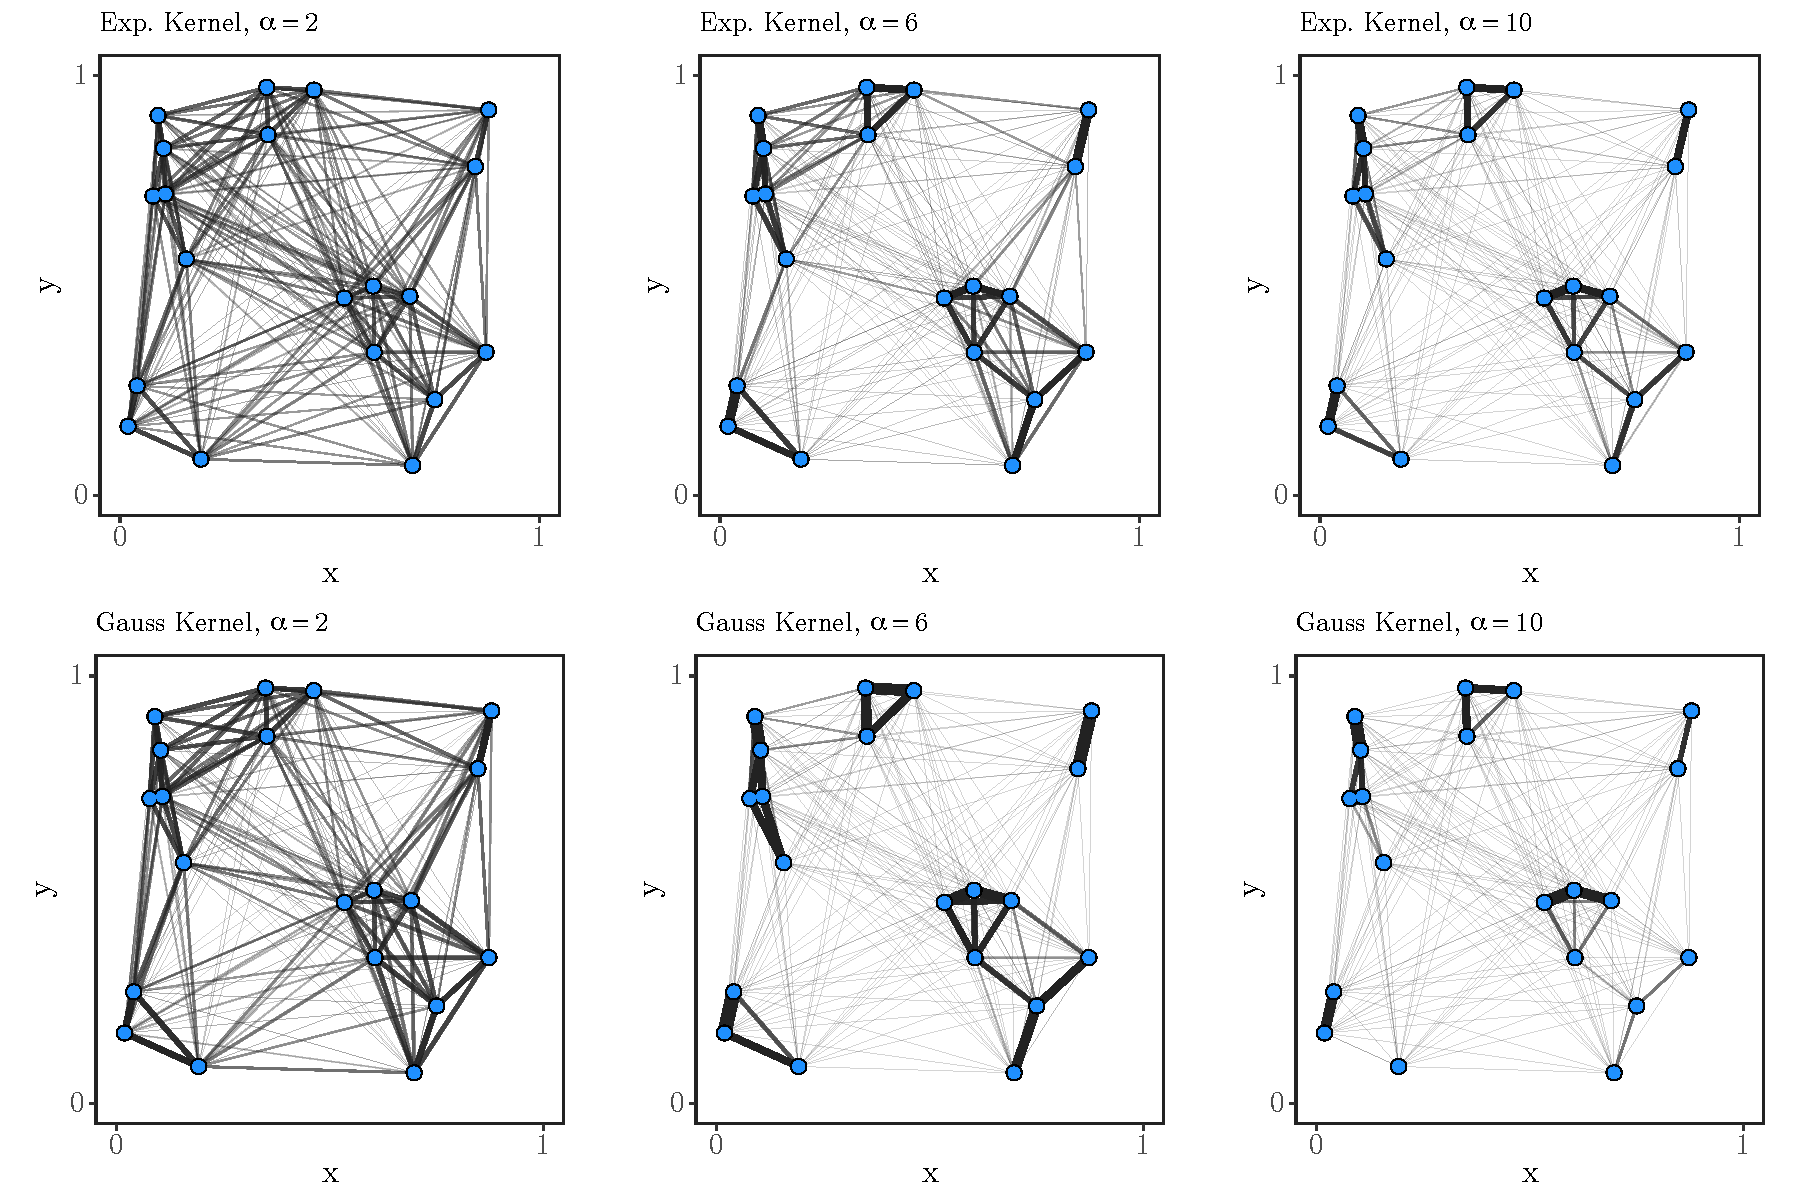
\includegraphics[width=15cm]{./figs/figure1}
		%Captions and Labels can be used since this is a figure environment
		\caption{Sample output from tikzDevice}	\label{fig:mp}
\end{figure}

Now that we have a model of landscape connectivity, we turn to defining a model of metapopulation dynamics on these spatial graphs.


\hypertarget{local-dynamics}{%
\subsection{Local Dynamics}\label{local-dynamics}}

We model population dynamics within each local population $L_i$ using
the stochastic logistic model. The dynamics of the number of individuals $N_i$
in population $L_i$  are described by the stochastic differential
equation (SDE)

\[dN_i=\lambda_i N_i \bigg(1 - \frac{N_i}{K_i}\bigg)dt+\sigma N_idW\]

Here, \(N_i\) is the abundance of population \(L_i\), \(\lambda_i\) is the
strength of density dependence in that population, and \(K_i\) is the
carrying capacity of \(L_i\). \(\sigma_p\) represents that standard
deviation in abundance due to local stochasticity as a proportion of
\(N_i\). Here \(\sigma\) represents an amalgamation of all factors
contributing to local stochasticity in population dynamics, although it
should be noted that the relative contribution of different factors to
local stochasticity can drive significant variation in dynamics
\cite{melbourne_extinction_2008}.


We can write this system as the matrix equation
\begin{equation}
        d\boldsymbol{N} = \boldsymbol{I} \boldsymbol{\lambda} \bigg(\boldsymbol{I}(\boldsymbol{K} - \boldsymbol{N})\boldsymbol{K}^{-1} \bigg) d\boldsymbol{t} + \boldsymbol{I} \boldsymbol{\sigma} \boldsymbol{N} d\boldsymbol{W}
\end{equation}


For the sake of reducing the size of parameter
space, here we consider all populations as having the same \(\lambda_i\)
and \(K_i\), however, future work could include exploring the
source-sink dynamics in this system by varying intrinsic growth rates
and carrying capacities across populations.

We use an SDE representation because they have been used to study phase
transitions in stochastic systems before \cite{brock_early_2012, kuehn_mathematical_2011}, and they have many nice properties for inference. SDEs
have also been used in ecology to study extinction dynamics before, as it is relatively straightforward to compute the mean time until extinction (MTE) using
the Kolmogorov Backward Equation \cite{lande_stochastic_2003}.

\hypertarget{diffusion-on-spatial-graphs}{%
\subsection{Diffusion on Spatial
Graphs}\label{diffusion-on-spatial-graphs}}

When we model a landscape with a spatial graph, we have to decide how
different nodes affect one another. The processes that connect
landscapes are inherently stochastic. The probability that an individual
migrates within its lifetime, $m$, and where it goes, $\Phi_{ij}$, are both stochastic . Under some conditions, we can
effectively model stochastic dynamics across space using diffusion
models. In essence, a diffusion model assumes that at each timestep the
system will change according to the expected value of stochastic
dispersal. Diffusion models have seen widespread use in ecology and
other fields \cite{ovaskainen_empirical_2008, holmes_partial-differential_1994, okubo_diffusion_2011}.

Given our dispersal potential $\Phi_{ij}$, we can define the
diffusion matrix \( D \) as

\[D_{ij} = \begin{cases} 1 - m \quad\quad &\text{if}\ i = j \\ \Phi_{ij}m & \text{if}\ i \neq j\end{cases}\]

We can now represent the
dynamics due to diffusion of this system as

\[\dot{N_i}=(1-m)N_i+ \sum_j \Phi_{ij}mN_j\]

In matrix notation, we can represent this diffusion model as

\[\frac{d\vec{N}}{dt}=D^T\vec{N}\]

We can then combine this with local dynamics as a reaction-diffusion
model,

\[\frac{d\vec{N}}{dt} = g(D^T \vec{N})\]

where \(g(x)\) is a function that represents the hypothesized mechanism
of how the ecological measurement evolves locally.


In principle, \(g(x)\) can represent any ecological process of
interest---for example if the state space of \(x\) is allelic
frequencies, \(g(x)\) could describe genetic drift, or if \(x\)
represents community compositions across space, \(g(x)\) could describe
competition between species as a function of environmental conditions,
coevolutionary states across space, etc. Here, we consider \(g(x)\) to
be the stochastic logistic model (see previous section). Combining this
with the diffusion model yields the SDE

\begin{equation} \label{diffusion_model}
  d \boldsymbol{N} = \boldsymbol{I} (D^T \boldsymbol{N})\bigg(\boldsymbol{I}\boldsymbol{K}^{-1}(\boldsymbol{K}-D^T \boldsymbol{N})\bigg) d\boldsymbol{t} + \boldsymbol{I}\boldsymbol{\sigma} \boldsymbol{N} \ d\boldsymbol{W}
\end{equation}

which will be the primary object of study in this paper.

\hypertarget{measuring-synchrony}{%
\subsubsection{Measuring Synchrony}\label{measuring-synchrony}}

As described above, measures of correlation in space and time are often
used in the study of phase transitions. When the order parameter gains
or loses correlation in space and time is used as an indicator of when a
system changes qualitative phases. Within the context of ecology, the
crosscorrelation function, \(CC\), has long been used as a measure of
synchronous dynamics \cite{liebhold_spatial_2004}. Here, with a subdivided
population, we consider the mean crosscorrelation compared across all
populations, \({PCC}=\frac{1}{n^2}\sum_{i,j} CC(V_i,V_j)\) . As an
example, in \ref{async_and_sync}, panel (a) show an example of low PCC,
and panel (b) shows an example of high PCC.

\begin{figure}[h]
\includegraphics[width=15cm]{./figs/figure2}
\caption{The abundance of 2 populations (top) and 8 populations (bottom) across time. Get the values of synchrony }
\label{async_and_sync}

\end{figure}

\hypertarget{simulating-a-phase-transition-across-a-migration-gradient}{%
\subsubsection{Simulating a Phase Transition across a Migration
Gradient}\label{simulating-a-phase-transition-across-a-migration-gradient}}

Now we consider how synchrony changes as a function of \(p_m\). Each run
consists of the following parameters,
\(\theta = \{N_p, \lambda, \sigma_p, \vec{K},p_m, \alpha \}\). For each
unique set of parameters, we run \(50\) replicates across all values of
\(p_m = \{0.01,0.02,\dots,1.0 \}\). For each replicate, we independently
draw the location of \(N_p\)     populations uniformly in \([0,1]^2\). We
draw the intial value of abundance for all populations from a uniform
distribution, \(N_i \sim U(0, K_i)\). We then integrate equation
\ref{diffusion_model} forward \(500\) timesteps using the
Euler--Maruyama method with \(\Delta t=0.1\). After integrating forward,
we compute the crosscorrelation coefficient, \(CC\) for each pair of
populations \(i \neq j\). Then, we compute the mean pairwise
crosscorrelation for that replicate, \(PCC\), and start the next
replicate.



\pagebreak
\begin{figure}
    \includegraphics[width=15cm]{figs/figure3}
    \caption{}
    \label{}
\end{figure}

\begin{figure}
    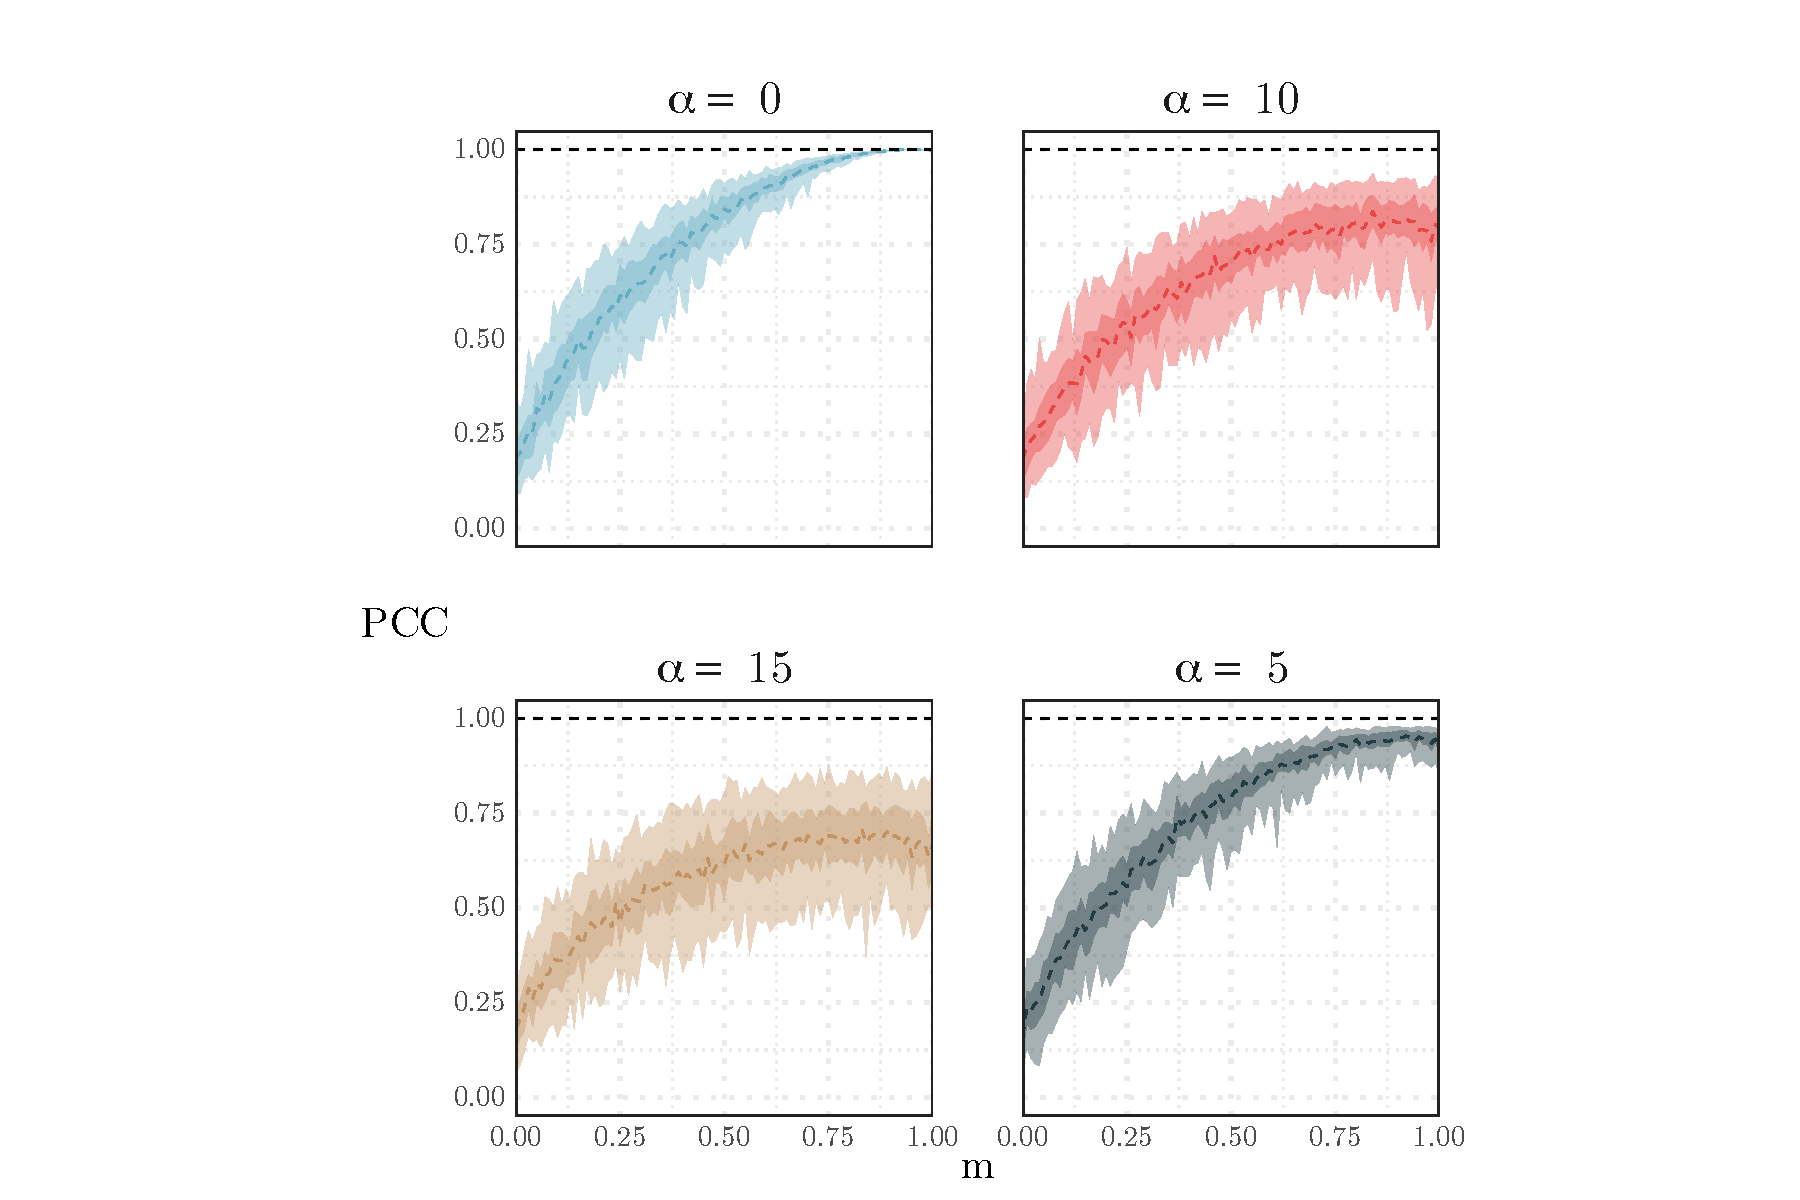
\includegraphics[width=15cm]{figs/figure4}
    \caption{}
    \label{}
\end{figure}


\begin{figure}
    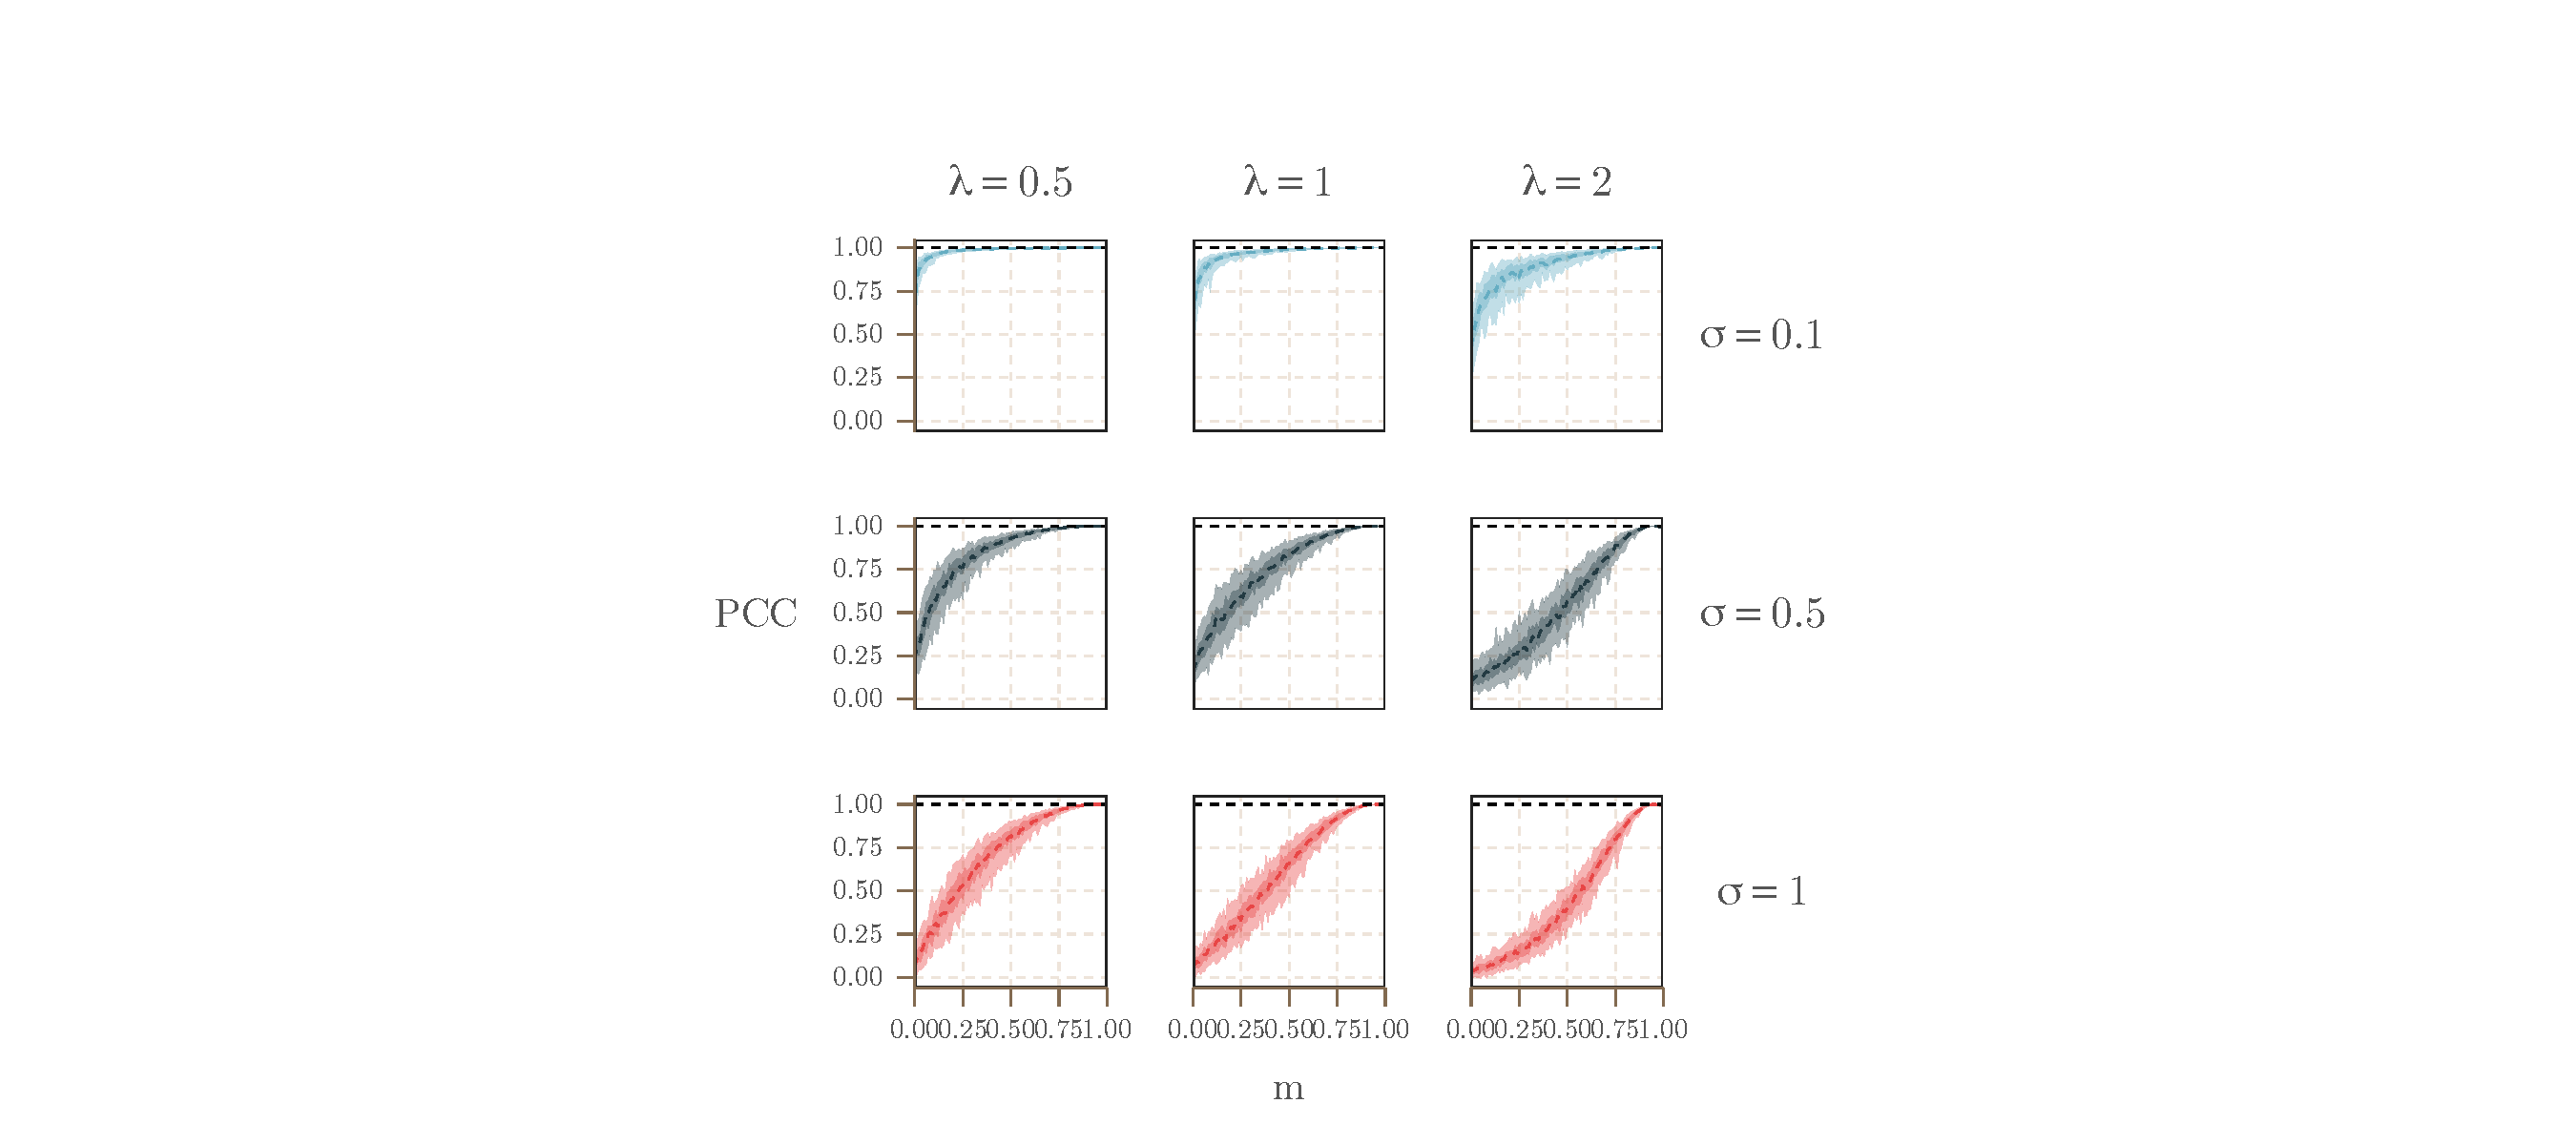
\includegraphics[width=15cm]{figs/figure5}
    \caption{}
    \label{}
\end{figure}


\clearpage
{
\footnotesize
\bibliography{references}
}



\end{document}
